\chapter{El átomo de helio}
Es un ejemplo de problema de tres cuerpos, no resoluble
analíticamente. En CGS\footnote{Sistema basado en el gramo, el segundo
y el centímetro. La ley de Coulomb es simplemente $1\cdot\frac{qq'}{r^2}$,
donde la distancia está en centímetros y la carga en \emph{estatculombios}.} el hamiltoniano se escribe como
\begin{equation}
   \Ham  = \frac{-\hbar^2}{2m} \nabla_1^2 - \frac{\hbar^2}{2m}
  \nabla_2^2 - \frac{Ze^2}{r_1} - \frac{Ze^2}{r_2} + \frac{e^2}{r_{12}}
  \label{eq:heliumh}
\end{equation}
donde $Z=2$ en el helio. Para el Li\textsuperscript{+} vale $Z=4$,
para el Be\textsuperscript{++} cinco, etc. Estamos suponiendo que la
masa del núcleo es mucho más grande que la masa del electrón.

Es un hamiltoniano de partículas idénticas, ya que permutar los
índices no lo varían. No obstante, hay un término de interacción que
no es eliminable por ser del mismo orden de magnitud\footnote{
Si comparamos los niveles experimentales del helio con el
    modelo suponiendo nulo el término de interacción
    electrón-electrón, vemos que la aproximación es mala:
    \begin{center}
      \includegraphics[width=0.4\textwidth]{figures/helium_noint.png}
    \end{center}
Los niveles en el caso de partículas independientes vienen dados
por \[E_{nn'} = -136 \left( \frac{Z^2}{n^2} + \frac{Z^2}{n'^2}
  \right) \text{ eV}\]
}. No obstante, podemos tratarlo como una perturbación para obtener
resultados analíticos.

La función de ondas resultante de esta aproximación ha de ser antisimétrica,
\begin{equation}
  \psi \propto \varphi_{n\ell m\mu}(1)\varphi_{n'l'm'\mu'}(2) - \varphi_{n\ell m\mu}(2)\varphi_{n'l'm'\mu'}(1)
\end{equation}
donde los números entre paréntesis indican en qué coordenadas evaluar las
funciones de ondas. Por ejemplo, $R(1)$ es notación para $R(r_1)$ y
$Y_{-1}^{1}(3)$ significa $Y_{-1}^1 (\Omega_3)$.

El factor de normalización de la función de ondas es simplemente
$\frac{1}{\sqrt{2}}$, ya que las $\varphi_i$ son ortogonales con las
$\varphi_{i'}$. En el caso en que los números cuánticos son iguales la
función de ondas ya no tiene esa norma (al no ser las $\varphi$
ortogonales, sino iguales), pero dichas funciones de onda están
prohibidas por el postulado de simetrización\footnote{En el caso de
  partículas no interactuantes, se puede recurrir al principio de
  exclusión de Pauli.}; el determinante de
Slater correspondiente tendría dos columnas iguales y sería nulo,
dando como resultado una función de ondas de norma nula.

\section{Nivel fundamental}
La función de ondas de este nivel, en la aproximación de electrones no
interactuantes, es
\begin{equation}
  \psi = \frac{1}{\sqrt{2}} [\varphi_{100\oh}(1) \varphi_{100\moh}(2)
  - \varphi_{100\oh}(2) \varphi_{100\moh}(1)]
\end{equation}
No hay degeneración. Podemos escribir $\psi$ como
\begin{equation}
  \begin{split}
    \psi &= \frac{\varphi_{100}(1)\varphi_{100}(2)}{\sqrt{2}}
    ( \ket{+}_1\ket{-}_2 - \ket{-}_1\ket{+}_2 ) \\
    &= \varphi_{100}(1)\varphi_{100}(2) \chi_0^0(1,2)
  \end{split}
\end{equation}
donde se ha utilizado una tabla de Clebsch-Gordan para escribir $
\frac{1}{\sqrt{2}}( \ket{+}_1\ket{-}_2 - \ket{-}_1\ket{+}_2 ) =
\chi_0^0(1,2)$. Vemos que hay simetría en la parte espacial y
antisimetría en la parte de los espines, de forma que la función de
ondas total es antisimétrica.

\subsection{Aproximación perturbativa}
Supongamos que el término $\frac{e^2}{r_{12}}$ es una perturbación.
Calculamos la corrección en primer orden a la energía del nivel
fundamental, el cual no es un nivel degenerado:
\begin{equation}
  \begin{split}
    \Delta E^{(1)} &=
    \ev{\frac{e^2}{r_{12}}}{\varphi_{100}(1)\varphi_{100}(2)\chi_0^0(1,2)} =
    \\
    &=
    \ev{\frac{e^2}{r_{12}}}{\varphi_{100}(1)\varphi_{100}(2)}\cancelto{1}{\ip{\chi_0^0(1,2)}}
    =\\ &=\cdots
  \end{split}
\end{equation}

Es muy incómodo trabajar con $r_{12}$ porque es un vector que no parte
del origen. Utilizando resultados de la electroestática clásica
escribimos:
\begin{equation}
  \frac{1}{r_{12}} = \sum_{\ell=0}^\infty \frac{r_<^\ell}{r_>^{\ell+1}} \text{P}_\ell(\cos\alpha)
\end{equation}
donde $r_<$ y $r_>$ son respectivamente el menor y el mayor de $r_1,r_2$
y $\text{P}_\ell$ es el polinomio de Legendre de orden $\ell$, que puede
escribirse en función de los armónicos esféricos como
\begin{equation}
  \text{P}_\ell (\cos \alpha) = \frac{4\pi}{2\ell+1} \sum_{m=-\ell}^l
  Y_\ell^{m*}(\Omega_1) Y_\ell^{m}(\Omega_2)
\end{equation}

A pesar de
haber eliminado $r_{12}$ de la integral tenemos que resolver una suma
infinita. Escribimos la parte espacial de la función de ondas como
\begin{equation}
  \varphi_{100}(\boldrm{r}_1) \varphi_{100}(\boldrm{r}_2) = \frac{Z^3}{\pi
    a_0^3} e^{\frac{-Z}{a_0}(r_1+r_2)}
\end{equation}
La integral, con todas las sustituciones, queda como
\begin{equation}
  \begin{split}
    \cdots &= \left( \frac{Z^3}{\pi a_0^3} \right)^2 e^{2}
    \iint_0^\infty r_1^2\dd{r_1}r_2^2\dd{r_2} \sum_{\ell=0}^\infty
    \frac{r_<^\ell}{r_>^{\ell+1}} e^{-2Z(r_1+r_2)/a_0} \cdot \\ &\cdot\sum_{m=-\ell}^\ell
    \frac{4\pi}{2\ell+1}\int_{4\pi} Y_\ell^{m*}(\Omega_1) \dd{\Omega_1}
    \int_{4\pi} Y_\ell^{m}(\Omega_2) \dd{\Omega_2} = \cdots
  \end{split}
\end{equation}
La integral contiene a dos armónicos esféricos ortogonales, así que
solo será no nula si $\ell=m=0$:
\begin{equation}
  \int_{4\pi}Y_\ell^{m*}(\Omega_1) \dd{\Omega_1} = \int_{4\pi}
  Y_\ell^m(\Omega_2) \dd{\Omega_2} = \sqrt{4\pi} \delta_{\ell0} \delta_{m0}
\end{equation}

Con ello, obtenemos:
\begin{equation}
  \cdots = \left( \frac{Z^3}{\pi a_0} \right)^2 e^{2} 16 \pi^2
  \iint_0^\infty r_1^2 \dd{r_1} r_2^2 \dd{r_2} \frac{1}{r_>}
  e^{-2Z(r_1+r_2)/a_0} = \cdots
\end{equation}
El siguiente paso es sustituir $r_>$ por la $r$ correspondiente en
cada región de integración. En $\int_0^\infty \dd{r_1} \int_0^{r_1} \dd{r_2}$ el mayor $r$
es $r_2$, y en $\int_0^\infty \dd{r_1} \int_{r_1}^\infty \dd{r_2}$ el
mayor pasa a ser $r_1$; conocido esto obtenemos:
\begin{equation}
  \begin{split}
    \cdots &= \left( \frac{Z^3}{\pi a_0} \right)^2 e^{2} 16
    \pi^2\int_0^\infty r_1^2 \dd{r_1} \Big[ \int_0^{r_1} \dd{r_2}
      \frac{1}{r_1} r_2^2 e^{-2Z(r_1+r_2)a_0} + \\ &+ \int_{r_1}^\infty
      \dd{r_2} \frac{1}{r_2} r_2^2 e^{-2Z(r_1+r_2)a_0} \Big] 
  \end{split}
\end{equation}

resolviendo las integrales resultantes, finalmente obtenemos
\begin{equation}
  \Delta E^{(1)} = \frac{5}{128} \frac{a_0^5}{Z^5}
  \stackrel{\text{He}}{=} \SI{34}{\eV}
\end{equation}
Vemos que la corrección es grande. El valor corregido (\SI{-74.8}{\eV})
es similar\jokenote{Que sean más o menos iguales depende de la
  escala, pero da igual porque la energía no es trabajo, que es lo que
es dinero. Y la pela es la pela, incluso en Panamá.} al experimental (\SI{-79}{\eV}).

\subsection{Aproximación variacional}

Ahora que conocemos la energía, podemos estimar la función de ondas
del nivel fundamental con el método variacional. Utilizamos una
función de prueba con un parámetro $\alpha$:
\begin{equation}
  \psi = \underbrace{\frac{\alpha^3}{\pi a_0^3} e^{-\alpha(r_1+r_2)/a_0}}_{\text{simmetric}} \underbrace{\chi_0^0(1,2)}_{\text{ant.}}
\end{equation}
$\alpha$ hace las veces de $Z$; de esta forma suponemos que bajo la
interacción los electrones se comportan como si fueran independientes
pero en un potencial central distinto a $Z=2$. Separamos $\psi$ en la
parte espacial y la de espín:
\begin{equation}
  \varphi =
  \varphi_{100}(\boldrm{r}_1,\alpha)\varphi_{100}(\boldrm{r}_2,\alpha) \chi_0^0
\end{equation}
Las $\varphi$ están en un potencial de Coulomb con $Z=\alpha$. Su forma
funcional es
\begin{equation}
  \varphi_{100}(\boldrm{r},\alpha) = \left( \frac{\alpha^3}{\pi a_0^3}
  \right)^{\oh} e^{-\alpha r /a_0}
\end{equation}
Las $\varphi$ son autoestados de $\frac{-\hbar^2}{m}\nabla^2 -\alpha
\frac{e^2}{r}$ con autovalor $\frac{-1}{2}\frac{e^2}{a_0}\alpha^2$.
Calculamos $\ev{ \Ham }{\psi}$ para tratar de minimizarlo, de esa
forma hallaremos la $\psi$ más parecida a $\psi_0$. Analizemos por
separado cada integral del hamiltoniano del helio \eqref{eq:heliumh}:
\begin{itemize}
\item Comenzamos por el término cinético:
  \begin{equation}
    \begin{split}
      \ev{\frac{-\hbar^2}{2m}\nabla_1^2}{\psi} &=
      \ev{\frac{-\hbar^2}{2m}\nabla_1^2}{\varphi_{100}(\boldrm{r}_1,\alpha)}
      \cdot \\ &\cdot \underbrace{\ip{\varphi_{100}(\boldrm{r_2},\alpha)}}_{=1}
      \underbrace{\ip{\chi_0^0}}_{=1}
    \end{split}
  \end{equation}
  Utilizando el teorema del virial obtenemos $\langle T \rangle = -E =
  \frac{+1}{2} \frac{e^2}{a_0} \alpha^2$. Con el término cinetico de
  la otra partícula ocurre lo mismo.
\item El término de potencial central resulta:
  \begin{equation}
    \begin{split}
      \ev{\frac{Ze^2}{r}}{\psi} &=
      \ev{\frac{-Ze^2}{r_1}}{\varphi_{100}(\boldrm{r}_1,\alpha)} \cdot \\
      &\cdot \underbrace{\ip{\varphi_{100}(\boldrm{r_2},\alpha)}}_{=1}
      \underbrace{\ip{\chi_0^0}}_{=1} = \\
      &= \frac{Z}{\alpha} \langle V \rangle
      \stackrel{\text{virial}}{=} \frac{Z}{\alpha} \underbrace{2 \left( \frac{-1}{2}\frac{e^2\alpha}{a_0} \right)}_{2E_0}
    \end{split}
  \end{equation}
\item Por último, calculamos\footnote{Se deja como ejercicio para el
    estudiante.} el término de interacción.
\begin{equation}
  \ev{\frac{e^2}{r_{12}}}{\psi} = \cdots = \frac{5}{8} \frac{\alpha e^2}{a_0}
\end{equation}
\end{itemize}

Si juntamos los resultados, obtenemos
\begin{equation}
  \ev{ \Ham }{f(\alpha)} = \frac{e^2}{a_0} \left(\alpha^2 -2Z\alpha +
    \frac{5}{8}\alpha \right)
\end{equation}
Vemos que el mínimo está en $\alpha = Z - \nicefrac{5}{16}$, con valor
$\SI{-77.5}{\eV} \geq E_0$ ($Z=2$). El valor experimental es
\SI{-78.8}{\eV}, y el perturbativo era \SI{-74.8}{\eV}. Como
$\eval{E_\text{var.}}_\text{min} \simeq E_\text{exp.}$ es plausible\jokenote{Tan plausible como que no tenemos otra.} que
$\psi(\alpha_\text{min}) \simeq \psi_0$. Por tanto, tenemos una
indicación de que es conveniente utilizar $Z=2-\nicefrac{5}{16}$ en
lugar de $Z=2$.

Con funciones de ondas más complicadas y más parámetros se pueden
sacar energías más cercanas a $E_0$ (y por tanto ajustar mejor
$\psi_0$). Hylleraas\historynote{Egil Andersen Hylleraas (1898-1965) fue un distinguido físico teórico
noruego conocido por su método simple pero elegante para predecir el
estado energético fundamental de átomos de dos electrones, así como
funciones de onda de prueba de átomos multielectrónicos. Hylleraas era
el nombre de la granja en que nació.} realizó un análisis especialmente
minucioso, obteniendo una diferencia con $E_0$ en la sexta cifra significativa.

\section{Niveles excitados}
Definimos un potencial central virtual $V(r)$ que nos permite escribir
el hamiltoniano del sistema como
\begin{equation}
  \begin{split}
     \Ham  = -\frac{\hbar^2}{2m}\nabla_1^2 -
      \frac{\hbar^2}{2m}\nabla_2^2 &+ V(r_1) + V(r_2)
    - \\
    &- V(r_1) - V(r_2) - \frac{\alpha e^2}{r_1} - \frac{\alpha
      e^2}{r_2} + \frac{e^{2}}{r_{12}} 
  \end{split}
\end{equation}

De esta manera tenemos el hamiltoniano expresado como un hamiltoniando
de partículas idénticas e independientes: 
\begin{align}
 \Ham _0 &= \frac{-\hbar^2}{2m}\nabla_1^2 - \frac{\hbar^2}{2m} \nabla_2^2 + V(r_1)
+ V(r_2) = h_1+h_2 \\
                W &=  - V(r_1) - V(r_2) - \frac{\alpha e^2}{r_1} - \frac{\alpha
      e^2}{r_2} + \frac{e^{2}}{r_{12}} \ll  \Ham _0
\end{align}
Cada partícula independiente cumple con $ \Ham _0$ la siguiente
ecuación de autovalores:
\begin{equation}
  \left[ \frac{-\hbar^2}{2m} + V(r) \right] \varphi_{n\ell m\mu}(\boldrm{r})
  = E_{nl} \varphi_{n\ell m\mu}(\boldrm{r})
\end{equation}
donde $\varphi_{n\ell m\mu}(\boldrm{r}) = R_{nl}(r) Y_l^m(\Omega)\ket{\oh\
  \mu}$, y el CSCO es $ \Ham ,L^2,L_z,S_z$.

Resolvemos la parte radial expresando $ \Ham _0$ en coordenadas
radiales en la ecuación de Schrödinger:
\begin{equation}
  \left[ \frac{-\hbar^2}{2m} \dv[2]{r} + V(r) + \frac{\ell (\ell+1)
      \hbar^2}{2mr^2}\right] = \chi_{n\ell}(\boldrm{r}) = E_{n\ell} \chi_{n\ell}(r)
\end{equation}
donde $\chi_{nl} = r R_{nl}$. El valor de $\ell$ cambia el tipo de
ondas que obtenemos como autoestados. Con $\ell =0$ obtenemos ondas de
tipo \emph{s} y energías $E_{1s},E_{2s},\ldots$, con $\ell = 1$ las
ondas son \emph{p} y las energías $E_{2p},E_{3p},\ldots$ etc. Se ha utilizado
el convenio de física atómica, donde se expresa la mínima $n$ como
$\ell +1$.

Los autovalores de $ \Ham _0$ serán $E_{nl}+E_{n'l'}$, al ser
partículas independientes. En notación de números de ocupación, los
autovalores son $(n\ell)^1(n'\ell')^1$. Los autoestados serían, en
principio,
$\varphi_{n\ell m\mu}(\boldrm{r}_1)\varphi_{n'\ell'm'\mu'}(\boldrm{r}_2)$, pero
necesitamos antisimetrizar la función de ondas por ser los electrones
fermiones:
\begin{equation}
  \Psi \propto  
\varphi_{n\ell m\mu}(\boldrm{r}_1)\varphi_{n'\ell'm'\mu'}(\boldrm{r}_2) - \varphi_{n\ell m\mu}(\boldrm{r}_2)\varphi_{n'\ell'm'\mu'}(\boldrm{r}_1)
\end{equation}


\subsection{Degeneración de los niveles}
\label{subsection:deglevel}

La degeneración de la energía para $E_{n\ell}\neq E_{n'\ell'}$ es distinta
que para el caso $E_{n\ell} = E_{n'\ell'}$:
\begin{itemize}
\item Si las energías son distintas,
 la degeneración corresponde al
  número de determinantes de Slater que podemos construir. Para
  construir un determinante de Slater necesitamos que los números
  cuánticos no sean exactamente iguales; dado un $\ell$ tenemos $2\ell +1$
  números distintos para la $m$ y $2s+1$ números para la $\mu$.
  Como el espín vale $\oh$ tenemos que $\mu = \pm \oh$, y tenemos que
  la degeneración es
  \begin{equation}
    g = \underbrace{(2\ell +1)}_{g_\ell} \cdot \underbrace{2}_{g_\mu} \cdot
    \underbrace{(2\ell' +1)}_{g_\ell'} \cdot \underbrace{2}_{g_\mu'}
  \end{equation}
\item Si las energías son iguales, los números cuánticos $\ell,\ell'$
  son idénticos y solo podemos variar $m,\mu$. Para $\ell=1$, por
  ejemplo, disponemos de seis\footnote{Concretamente,
    $m\in -\ell,\cdots,\ell$ y $\mu = \pm \oh$:
  \begin{center}
    \begin{tabular}{c|c}
     $\mu$ & $m$ \\ \hline
      $+\oh$ & $+1$ \\ 
      $+\oh$ & $\ \ 0$ \\ 
      $+\oh$ & $-1$ \\ 
      $-\oh$ & $+1$ \\ 
      $-\oh$ & $\ \ 0$  \\ 
      $-\oh$ & $-1$ \\ 
    \end{tabular}
  \end{center}
}
parejas de valores:
Tenemos que escoger grupos de dos parejas distintos para los estados.
Por ejemplo, $\ket{m\mu}=\ket{+1\ +\oh}$ y $\ket{m'\mu'}=\ket{0\ -\oh}$.
Hay seis parejas $(m,\mu)$ distintas, así que podemos escoger
$g=\binom{6}{2}$ estados distintos. Para $\ell$ genérica, la
degeneración será
\begin{equation}
  g = \binom{(2\ell + 1)\cdot 2}{2}
\end{equation}
\end{itemize}

Vemos que la degeneración puede crecer mucho, por lo que es importante
escoger buenas bases. 

\paragraph{Ejemplos}
\begin{itemize}
\item $E_{1s}+E_{2s} \ \rightarrow \ (1s)^1(2s)^1$. Las energías son
  distintas, así que hay $2\cdot(2\ell+1)\cdot 2 \cdot (2\ell'+1)$
  estados distintos. Como los orbitales \emph{s} se caracterizan por
  tener un número cuántico $\ell$ nulo, nos queda $2\cdot(0+1)\cdot 2
  \cdot (0+1)$ y obtenemos $g=4$.
\item $E_{1s}+E_{2p} \ \rightarrow \ (1s)^1(2p)^1$. En este caso
  aparece un orbital \emph{p}, con $\ell = 1$. Obtenemos $2\cdot(0+1)\cdot 2
  \cdot (2\cdot 1+1)$, y por tanto $g = 12$.
\item $2E_{1s} \ \rightarrow \ (1s)^2$. Las energías son iguales, así
  que la degeneración vendrá dada por $\binom{(2\ell +1)\cdot 2}{2}$.
  Como $\ell =0$, tenemos $g=\binom{2}{2}=1$.
\item $2E_{1p} \ \rightarrow \ (1p)^2$. En este caso $\ell =1$ y obtenemos 
  $g=\binom{2(2\cdot1 +1)}{2}=\binom{6}{2}=15$.
\end{itemize}

\subsection{Diagonalización de $W$}
Recordamos que
\begin{equation}
  W = -V(r_1) - V(r_2) - \frac{Ze^2}{r_1} - \frac{Ze^2}{r_2} + \frac{e^2}{r_{12}}
\end{equation}
No conmuta con rotaciones de una sola partícula\footnote{Es obvio, ya
  que si rotamos solo una partícula puede cambiar la distancia
  $r_{12}$ entre ambas.}, $\boldrm{L}_i$,
pero sí con rotaciones del sistema, $\boldrm{L} =
\boldrm{L}_1+\boldrm{L}_2$. $W$ no depende de los espines, así que
conmuta con todos sus operadores. En resumen, 
\begin{equation}
  [W,\boldrm{L}]=[W,\boldrm{S}]=[W,L_z]=[W,L^2] = 0
\end{equation}
Es posible que $L^2,L_z,S^2,S_z$ sean un CSCO para las
funciones antisimétricas del subespacio de degeneración
$E_{n\ell}+E_{n'\ell'}$, pero existe ambiguedad en la función. 
Sean dos parejas fijas de
números cuánticos $(n\ell)$ y $(n'\ell')$, los coeficientes de
Clebsch-Gordan nos dan dos funciones globales para el sistema,
$F_{\ell\ell'}\ket{M_L\ L}(\boldrm{r}_1,\boldrm{r}_2)$ y la
permutación $F_{\ell\ell'}\ket{M_L\ L}(\boldrm{r}_2,\boldrm{r}_1)$,
que pueden ser simétricas ($L$ par) o antisimétricas ($L$ impar).
Además, como parte de espín, podemos escoger\footnote{No hay más combinaciones, ya
  que con espín $\oh$ podemos obtener únicamente las combinaciones
  dadas por $\frac{1}{2} \otimes \frac{1}{2} = 0,1$. La demostración
  de que $S=0$ es antisimétrica y $S=1$ simétrica es inmediata
  escribiéndolos como combinación lineal en la base de
  $\ket{\pm}_1,\ket{\pm}_2$ con las tablas de Clebsch-Gordan y viendo
  que pasa al permutar los índices.} tanto  $\chi_0^0(1,2)$ (antisimétrica) y
$\chi_1^{M_S}(1,2)$ (simétrica). Esto nos da una degeneración doble
por la elección del espín,
pero es solventable con el postulado de simetrización. Escribimos
ambas posibles funciones del sistema como
\begin{equation}
  \Psi =
  \begin{cases}
&F_{\ell\ell'} {M_L \atop L}(\boldrm{r}_1,\boldrm{r}_2) \chi_0^0(1,2)\ 
\pm  \
F_{\ell\ell'}{M_L\atop L}(\boldrm{r}_2,\boldrm{r}_1) \chi_0^0(1,2) \\
&F_{\ell\ell'} {M_L \atop L}(\boldrm{r}_1,\boldrm{r}_2) \chi_1^{M_S}(1,2)\ 
\pm  \
F_{\ell\ell'}{M_L\atop L}(\boldrm{r}_2,\boldrm{r}_1) \chi_1^{M_S}(1,2) 
  \end{cases}
  \label{eq:psicases}
\end{equation}

donde el $\pm$ depende de si la función $F$ era simétrica o
antisimétrica\footnote{Si son simétricas basta con sumarlas, si son
  antisimétricas hemos de restar su permutación.}.
Vemos que hay dos elecciones posibles debido a $\chi$, pero que $\Psi$ tenga que ser
antisimétrica lo soluciona.
\begin{itemize}
\item Si $L$ es par, la función $F_{\ell\ell'}{M_L \atop L}$ ha de tener parte de espín antisimétrica,
  $\chi_0^0(1,2)$. De esta forma, obtenemos $\text{sim}\otimes
  \text{antisim} = \text{antisim}$.
\item Si por el contrario $L$ es impar, la función ha de tener parte
  de espín par, $\chi_1^{M_S}(1,2)$. Así se obtiene $\text{antisim}\otimes
  \text{sim} = \text{antisim}$.
\end{itemize}

De esta forma podemos escoger uno de los dos casos de la
ecuación \eqref{eq:psicases}, y vemos que el CSCO es realmente
completo. Notar que todo este tratamiento es válido únicamente para
sistemas de
dos partículas. Obtenemos una representación matricial completamente
diagonal para $W$:
\begin{equation}
  \ev{W}{\Psi} \sim
  \delta_{\ell\ell'}\delta_{M_L M_L'}\delta_{S^2 S'^2}\delta_{M_S M_S'}
\end{equation}
donde $\ket{\Psi}  = \ket{(n\ell)(n'\ell')L\ M_L\ S\ M_S}$.

En principio se tendría que calcular todos los valores de la diagonal,
pero como se vio en los ejercicios\footnote{Estructura fina del hidrógeno,
  sección de la página \pageref{paragraph:l0vm}, ecuación \ref{eq:exercises_recurrence}}
el hecho de que $[V,\boldrm{J}]=\boldrm{0}$ implica que $\ev{V}{\alpha j m}
= \ev{V}{\alpha j m\pm 1}$. En principio no esperamos que aparezca el
espín, pero lo tenemos en cuenta. 

\subsection{Términos espectroscópicos}
Tenemos energías del estilo $E = E_{n\ell}+E_{n'\ell'}+\Delta(n\ell n'\ell' L S)$. Si
solo indicamos la configuración, $(nl)(n'\ell')$, solo damos
información sobre $\Ham$ (en $n$) y $L^2$ (en $\ell$). El CSCO requiere
de más observables para ser completo, así que introducimos los
llamados \emph{términos espectroscópicos} para dar información sobre
los observables $L_z,S^2$ y completar el CSCO\footnote{Aún falta
  información sobre $S_z$, por lo que las configuraciones con término
  espectroscópico pueden seguir estando degeneradas.}.

Como ejemplo práctico, veamos la configuración $(1s)(2s)$. Tenemos un
valor único para $L$ en $0\otimes0 = \{0_S\}$ y dos para el observable espín
total, $S\in \oh \otimes \oh = \{0_S,1_A\}$, donde el subíndice indica si la
función es simétrica o no. Tenemos por tanto dos parejas, $\ket{L:0\
  S:0}$ y $\ket{L:0 \ S:1}$, para indicarlas introducimos un término
 extra ${}^{2S+1}L$, que nos da información del
momento angular orbital (en este caso sólo puede ser nulo) y el espín
total (uno o cero). Se utiliza la notación $S=0,P=1,D=2,F=3,\ldots$
para indicar $L$. Así pues, identificamos $\ket{L:0\ S:0}$ con un
estado \emph{singlete} ${}^{1}\!S$ y $\ket{L:0\ S:1}$ con ${}^3\!S$ 
(\emph{triplete}). La degeneración de cada subestado es simplemente
$2S+1$, como puede verse en el diagrama de niveles de la figura \ref{fig:uncoupling}.


\begin{marginfigure}
  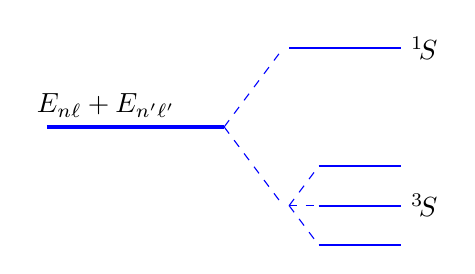
\begin{tikzpicture}[xscale=1.5,yscale=1]
    \draw[blue, ultra thick] (0,1) -- (1.5,1);
    \draw[blue, thin, dashed] (1.5,1) -- (2,2);
    \draw[blue, thick] (2.05,2) -- (3,2);
    \draw[blue, thin, dashed] (1.5,1) -- (2,0);
    \draw[blue, thick] (2.3,0) -- (3,0);
    \draw[blue, thick] (2.3,0.5) -- (3,0.5);
    \draw[blue, thick] (2.3,-0.5) -- (3,-0.5);
    \draw[blue, thin, dashed] (2.05,0) -- (2.3,0);
    \draw[blue, thin, dashed] (2.05,0) -- (2.3,0.5);
    \draw[blue, thin, dashed] (2.05,-0) -- (2.3,-0.5);
    \draw node [above] at (0.5,1) {$E_{n\ell}+E_{n'\ell'}$};
    \draw node [right] at (3,2) {${}^1\!S$};
    \draw node [right] at (3,0) {${}^3\!S$};
  \end{tikzpicture}
  \caption{Degeneración de los niveles del helio}
  \label{fig:uncoupling}
\end{marginfigure}

Notar que obtenemos la misma degeneración ($1+3$) que si aplicamos las
fórmulas de \ref{subsection:deglevel}

\paragraph{Términos espectroscópicos}
Cada nivel $E_{n\ell}+E_{n'\ell'}$ tendrá como degeneración el número de
parejas $L,S$. Por ejemplo, para el nivel $(1s)(2s)$ tenemos
que $L\in\{0\otimes0\}=\{0_S\}$ y
$S\in\{\oh\otimes\oh\}=\{0_A,1_S\}$. El estado electrónico no queda
completamente determinado con la notación $(1s)(2s)$, lo que nos hace
incluir un término extra ${}^{2S+1}L$, que nos da información\footnote{El CSCO completo requiere de
  $L^2,L_z,S^2,S_z$,y el término espectroscópico añade información
  sobre $S_z$. Por ejemplo, el estado $(1s)(2s)\ {}^3\!S$ está triplemente
degenerado, ya que falta por indicar $S_z$.} del
momento angular orbital (en este caso sólo puede ser nulo) y el espín
total (uno o cero). Se utiliza la notación $S=0,P=1,D=2,F=3,\ldots$
para indicar $L$. Por ejemplo, ${}^3\!S$ indica un estado
\emph{triplete}, que tiene un espín total uno y momento angular
orbital nulo.




\paragraph{Ejemplos}
\label{paragraph:examplesdegantisim}
\begin{description}
\item[(1s)(2p)] La degeneración del orbital $(1s)$ es doble (espín
  \emph{up} y \emph{down}) y la del $(2p)$ séxtuple (espín \emph{up} y
  \emph{down}, además de un factor $3$ por el momento angular
  orbital). En forma de tabla:
  \begin{center}
    \begin{tabular}{ccccc}
      deg. & $L$ & $S$ & ${}^{2S+1}\!L$ & deg. \\ \hline
      12   & $0\otimes1 = \{1\}$ & $0,1$ & ${}^{1}\!P, {}^{3}\!P$ & $3 +3\cdot 3$ \checkmark
    \end{tabular}
  \end{center}
  De forma general, la degeneración de ${}^{2S+1}\!L$ es $(2S+1)(2L+1)$.
\item[(2p)\textsuperscript{2}] Al tener ambos electrones la misma
  energía hemos de tener cuidado con que la función total sea
  antisimétrica\footnote{
    Si tenemos dos energías y dos funciones de onda espaciales distintas, como por ejemplo
    $(1s)(2p)$, la función de ondas global $\Psi(\boldrm{1},\boldrm{2})$ es
    $R_{1s}(\boldrm{1})Y_0^0(\boldrm{1})R_{2p}(\boldrm{2})Y_1^{+1}(\boldrm{2})$,
    que no es ni antisimétrica ni simétrica. Si necesitamos una
    función de ondas simétrica, podemos emplear
    $\Psi(\boldrm{1},\boldrm{2})+\Psi(\boldrm{2},\boldrm{1})$ y si la
    necesitamos antisimétrica
    $\Psi(\boldrm{1},\boldrm{2})-\Psi(\boldrm{2},\boldrm{1})$.

    En cambio, si tenemos la misma función de ondas (la misma energía), como en el caso
    $(1s)^2$, la función de ondas global es
    $R_{1s}(\boldrm{1})Y_0^0(\boldrm{1})R_{1s}(\boldrm{2})Y_0^0(\boldrm{2})$,
    que ya es simétrica. Si tratamos de antisimetrizarla, obtenemos $\Psi
    = 0$. En general, dado el orbital $(n\ell)^2$ la parte espacial de la
    función total $F_L^{M_L}$ permuta como
    \begin{center}
      \begin{tabular}{c|l}
        \text{Sim.} & $L=2\ell$ \\
        \text{Antisim.} & $L=2\ell-1$ \\
         $\cdots$      &  $\cdots$     \\
        \text{Sim.} & $L=0$ \\
      \end{tabular}
    \end{center}
}. La degeneración debería ser
  (utilizando \ref{subsection:deglevel}) $g=\binom{6}{2}=15$, y en
  efecto:
  \begin{center}
    \begin{tabular}{ccccc}
      deg. & $L$ & $S$ & ${}^{2S+1}\!L$ & deg. \\ \hline
      15   & $1\otimes1 = \{0_S,1_A,2_S\}$ & $0_A,1_S$ & ${}^{1}\!S,
                                                   {}^{1}\!D,
                                                   {}^{3}\!P$ & $1 +5+ 9$ \checkmark
    \end{tabular}
  \end{center}
  Obtenemos una matriz $15\times15$, de la que sólo tres autovalores son
  distintos. Notar que hemos dejado fuera combinaciones como $L:0_S +
  S:1_S = {}^{3}\!S$ por no ser antisimétricas.
\item[(2p)(3p)] La degeneración debería ser $36$. En efecto:
  \begin{center}
    \begin{tabular}{ccccc}
      deg. & $L$ & $S$ & ${}^{2S+1}\!L$ & deg. \\ \hline
      36   & $1\otimes1 = \{0_S,1_A,2_S\}$ & $0_A,1_S$ & ${}^{1}\!S,
                                                   {}^{1}\!D,
                                                   {}^{1}\!P$ & $1 +3+5+$ \\
       &  &  & ${}^{3}\!S,{}^{3}\!P,{}^{3}\!D$ &   $+3+9+15 $ \checkmark\\
    \end{tabular}
  \end{center}
  Vemos que el poder antisimetrizar a placer la parte espacial nos da
  muchas más posibilidades que en $(2p)(2p)=(2p)^2$. 
\end{description}



\paragraph{Integrales de intercambio}
\label{paragraph:intinterc}
Se ha visto como el término espectroscópico ${}^{2S+1}\!L$ depende del
espín. Es extraño, ya que la perturbación no depende de él. Calculemos
explícitamente la variación de energía $\Delta E$ en
\begin{equation}
  \begin{split}
    E &= E_{n\ell} + E_{n'\ell'} + \Delta(n\ell,n'\ell',L,S) = \\
    &= E_{n\ell} + E_{n'\ell'} + \\ &+ \ev{W(\boldrm{r}_1,\boldrm{r}_2)}{(n\ell)(n'\ell')LM_LSM_S}
  \end{split}
\end{equation}

Teniendo en cuenta la antisimetrización de la función (que cambia el signo
$\pm$ de la parte espacial en función de la simetría del espinor) se
obtiene:
\begin{fullwidth}
\begin{equation}
  \begin{split}
    \Delta E &=
    \ev{W(\boldrm{r}_1,\boldrm{r}_2)}{\frac{1}{\sqrt{2}}[F_L^{M_L}(\boldrm{r}_1,\boldrm{r}_2)\pm
      F_L^{M_L}(\boldrm{r}_2,\boldrm{r}_1)]\chi_S^{M_S}} = \\
    &= \ev{W(\boldrm{r}_1,\boldrm{r}_2)}{\frac{1}{\sqrt{2}}[F_L^{M_L}(\boldrm{r}_1,\boldrm{r}_2)\pm
      F_L^{M_L}(\boldrm{r}_2,\boldrm{r}_1)]}
    \underbrace{\ip{\chi_S^{M_S}}}_{=1}= \\
    &= \frac{1}{2} \ev{W}{F_L^{M_L}(\boldrm{r}_1,\boldrm{r}_2)}
    + \frac{1}{2} \ev{W}{F_L^{M_L}(\boldrm{r}_2,\boldrm{r}_1)}
    \pm \\ &\pm \left( 
    \frac{1}{2} \mel{F_L^{M_L}(\boldrm{r}_1,\boldrm{r}_2)}{W}{F_L^{M_L}(\boldrm{r}_2,\boldrm{r}_1)}
    + \frac{1}{2}
    \mel{F_L^{M_L}(\boldrm{r}_2,\boldrm{r}_1)}{W}{F_L^{M_L}(\boldrm{r}_1,\boldrm{r}_2)}  \right)
  \end{split}
\end{equation}
\end{fullwidth}

Eliminando casi toda la notación, para hacer la ecuación comprensible
para humanos:

\begin{equation}
  \begin{split}
    \Delta E &=
    \ev{W(\boldrm{1},\boldrm{2})}{\frac{1}{\sqrt{2}}[(\boldrm{1},\boldrm{2})\pm
      (\boldrm{2},\boldrm{1})]} = \\
    &= \frac{1}{2} \ev{W}{(\boldrm{1},\boldrm{2})}
    + \frac{1}{2} \ev{W}{(\boldrm{2},\boldrm{1})}
    \pm \\ &\pm
    \left( \frac{1}{2} \mel{(\boldrm{1},\boldrm{2})}{W}{(\boldrm{2},\boldrm{1})}
    + \frac{1}{2}
    \mel{(\boldrm{2},\boldrm{1})}{W}{(\boldrm{1},\boldrm{2})} \right)
  \end{split}
\end{equation}

Recordar que el signo del $\pm$ depende de la simetrización de la
función. Como las integrales son invariantes ante una transposición $1
\leftrightarrow 2$ y $W(\boldrm{1},\boldrm{2}) =
W(\boldrm{2},\boldrm{1})$, obtenemos que los cuatro sumandos son
iguales por parejas. Por tanto, $\Delta E = D \pm C$, donde $D$ es la
\emph{integral directa} y $C$ es la \emph{integral de intercambio}.

Vemos que el término de espín $\chi$ ha desaparecido, pero influye en $\Delta
E$ mediante el signo $\pm$. Si $S=0$ el signo es positivo y si $S=1$
es negativo\footnotemark; a esto se le llama \emph{correlación del intercambio con
el espín}.


En caso de ser las energías $E_{n\ell}$ y $E_{n'\ell'}$ iguales,
desaparecen los términos cruzados y $C=0$.

\section{Estructura fina}
Quedan varias interacciones en el hamiltoniano del sistema que aún no
se han tratado:
\begin{center}
  \begin{tabular}{lr}
     Término de masa& \\
     Término de Darwin& \\
    Término de
    espín-órbita&
                  $\boldrm{l}_1\boldrm{s}_1 + \boldrm{l}_2 \boldrm{s}_2$ \\
    Término de
    espín-espín&
                 $\boldrm{s}_1 \boldrm{s}_2$ \\
      Interacción del espín con
      la otra órbita  &
    $\boldrm{l}_1\boldrm{s}_2 + \boldrm{l}_2 \boldrm{s}_1$ \\
    Interacción
    órbita-órbita &
                   $\boldrm{l}_1\boldrm{l}_2$ \\
  \end{tabular}
\end{center}

Hay bastantes más que en el hidrógeno al tratarse de un sistema más
complejo. El término dominante, no obstante, es el de espín-órbita
para $Z>2$ (en el helio es dominante el de espín-espín). Además,
faltaría el término de \emph{efecto Lamb}\footnote{Acoplamiento con
  fluctuaciones del campo electromagnético del vacío} y la estructura
hiperfina (interacción con el momento magnético del núcleo).

En resumen, se tiene
\begin{equation}
  \Ham = \Ham_0 + W + W_\text{fine}
\end{equation}
donde esperamos que $W_\text{fine} \ll W$.


Sabemos que $W$ es diagonal en $\ket{n,\ell,n',\ell',L,M_L,S,M_S}$, pero
$W_\text{fine}$ no\footnote{Por ejemplo,
  $[W_\text{fine},\boldrm{L}]\neq \boldrm{0}$}; como sí que conmuta con
$\boldrm{J}$ nos planteamos utilizar la base
$\ket{n,\ell,n',\ell',L,S,J,M}$ de autoestados de $L^2,S^2,J^2,J_z$ en
$(n\ell)(n'\ell')$.\footnote{Si bien no se demuestra, $L^2,S^2,J^2,J_z$ es
  CSCO dados unos $(n\ell)(n'\ell')$ fijos, y las $\Psi$ resultantes son
  completamente antisimétricas.}

De la conmutación con $\boldrm{J}$ de $W_\text{fine}$ deducimos que
\begin{equation}
  \ev{W_\text{fine}}{(n\ell)(n'\ell')LSJM} \propto \delta_{JJ'}\delta_{MM'}
  \label{eq:conmutationef}
\end{equation}
Pero no podemos garantizar proporcionalidad con $\delta_{LL'}\delta_{SS'}$ ya
que los conmutadores no son nulos\footnote{La demostración se omite
  por ser tediosa}. La matriz no será del todo diagonal, pero sí algo;
en resumen:
\begin{align}
  W &=
  \begin{pmatrix}
    a& & & \\
     &b& & \\
     & &c& \\
     & & &\ddots \\
  \end{pmatrix} \ \ \ \text{in}\ \  \ket{(n\ell)(n'\ell')LM_LSM_S}\\
  W_\text{fine} &=
  \begin{pmatrix}
    a&\times&\times&\times \\
    \times&b&\times&\times \\
    \times&\times&c&\times \\
    \times&\times&\times&\ddots \\
  \end{pmatrix} \ \ \ \text{in}\ \  \ket{(n\ell)(n'\ell')LSJM}
\end{align}
Las $\times$ simbolizan que hay una diagonal fuerte pero algunos elementos
fuera de ella no son nulos. Es tentador sumar ambas matrices y
diagonalizar el resultado para resolver la estructura fina del helio,
pero están en distintas bases, por lo que no pueden
sumarse\jokenote{Ni Obama.}. Para poder hacerlo, veamos que $W$
es también diagonal en $\ket{(n\ell)(n'\ell')LM_LSM_S}$, de forma que estén
en la misma base. Empezamos por ver que
\begin{equation}
  [W,\boldrm{L}]=[W,\boldrm{S}]=0 \ \rightarrow \ [W,\boldrm{J}]=0
\end{equation}
Veamos cuánto valen sus elementos no nulos en la nueva base. Para
ello, utilizamos los coeficientes de Clebsch-Gordan\footnote{Recordar
  que estos coeficientes proyectan elementos de la base en
  $L^2,L_z,S^2,S_z$ a la base en $L^2,S^2,J^2,J_z$. Por ello, se
  emplea la notación $(LM_LSM_S|LSJM)$.}, efectuando el cambio


\begin{equation}
  \begin{split}
    \ket{(n\ell)(n\ell)LSJM} &\rightarrow  \underbrace{(LM_LSM_S|LSJM)}_{C_\ell}\ket{(n\ell)(n\ell)LM_LSM_S}\\
    \ket{(n\ell)(n'\ell')LSJM} &\rightarrow
    \underbrace{(LM_L'SM_S'|LSJM)}_{C_{\ell'}}\ket{(n\ell)(n\ell)LM_L'SM_S'}
  \end{split}
\end{equation}

Obtenemos que en la nueva base $\Delta E$ es
\begin{equation}
  \begin{split}
    &\mel{(n\ell)(n'\ell')LSJM}{W}{(n\ell)(n\ell)LSJM} = \\
    &= \sum_{\mathclap{M_L,M_S,M_L',M_S'}}
    C'_{\ell'}\ C_{\ell} \underbrace{\mel{(n\ell)(n'\ell')LM_L'SM_S'}{W}{(n\ell)
        (n\ell)LM_LSM_S}}_{\Delta(n\ell n'\ell'LS)\delta_{M_L,M_L'}\delta_{M_S,M_S'}}= \\
    &= \Delta E \cdot \sum_{M_L,M_S}
    \abs{\text{Clebsch-Gordan}}^2 = \Delta E \cdot 1\\
  \end{split}
\end{equation}

donde la $\Delta(n\ell n'\ell' L S)$ ha salido factor común de la suma al no
depender de los índices de esta. Vemos que los elementos de matriz de
$W$ en la nueva base son los mismos, y estamos listos para sumar ambas
matrices sin problemas.

\paragraph{Ejemplo: (1s)(2p)} La composición de $L$ resulta $L \in 0\otimes1
= \{1\}$, mientras que $S$ es $S\in \oh \otimes \oh = \{0,1\}$. La suma de
$L,S$ será\footnote{$J$ va desde $L_\text{min}=0$ hasta
  $L_\text{max}=2$ en saltos de $1$.} $J\in\{0,1,2\}$. La
degeneración de esta energía es $2\cdot 6$, así que la matriz será
$12\times12$; tendremos que calcular $144$ elementos a
priori\footnote{Sobran la mitad de los cálculos por ser la matriz hermítica}. Tenemos dos términos espectroscópicos, el ${}^{1}\!P$ y el
${}^{3}\!P$; veamos que elementos fuera de la diagonal\footnote{Por
  eso utilizamos distintos términos espectroscópicos en cada lado. Si
  no, estaríamos en la diagonal de la matriz.} no son
nulos\footnote{Para ser no nulos tenemos que tener las mismas $J,M$ a
  ambos lados (ver ecuación \eqref{eq:conmutationef}).}:
\begin{equation}
  \begin{split}
    \mel{(1s) (2p)\ {}^1\!P\ J\ M}{W_\text{fine}}{(1s) (2p)\ {}^3\!P\
      J\ M} &\neq 0\\
    \mel{
    (1s) (2p)\ {}^1\!P\ 
    \underset{1}{\overset{1}{\scriptstyle 1}} \ 
    \underset{-1}{\overset{+1}{\scriptstyle \  0}}
    }
    {
    W_\text{fine}
    }{
    (1s) (2p)\ {}^3\!P\
    \underset{1}{\overset{1}{\scriptstyle 1}} \ 
    \underset{-1}{\overset{+1}{\scriptstyle \ 0}}
    }
    &\neq 0
  \end{split}
\end{equation}
donde se ha utilizado que $J=1$ es la única $J$ que coincide en
ambos términos espectroscópicos. Vemos, por tanto, que sólo tres
elementos de fuera de la diagonal no son nulos\footnote{Más otros tres
al otro lado de la diagonal}.

Los términos de fuera de la diagonal son despreciables. Puede verse en
caso sencillo sumando a una matriz diagonal $\smqty(A&0\\ 0&B)$ una matriz
$\smqty(a&c^*\\ c &b)$ con $c\ll (a-b)^2$. 
Desarrollando en serie los
autovalores de la matriz suma vemos que las correcciones de los
elementos de la diagonal son pequeñas:
\begin{equation}
  \mqty(A& \\ & B) + \mqty(a&c^* \\ c & b) \sim \mqty(A+a & \\ & B+b)
  \label{eq:twobytwoargument}
\end{equation}

Con los valores típicos del
helio son menores de \SI{1e-7}{\eV}. A esta aproximación resultante de
suponer nulos estos elementos se le conoce
como \emph{acoplamiento LS} o de \emph{Rusell-Saunders}.

La energía a primer orden, por tanto, será
\begin{equation}
  E \simeq E_{n\ell} + E_{n'\ell'} + \Delta(n\ell n'\ell' LS) + \Delta_\text{fine}(n\ell n'\ell' LSJ)
\end{equation}
El término nuevo no depende de $M$ porque
$[W_\text{fine},\boldrm{J}]=0$. Esta energía está
degenerada $2J+1$
veces\footnote{Como $[W_\text{fine},\boldrm{J}]=0$ no depende de $M$,
  y la degeneración de $M$ es $2J+1$.}. 


Con todo lo visto, podemos razonar el desdoblamiento de un nivel como
el $(1s)(2p)$, por ejemplo (figura
\ref{fig:heliumlevelfinal}).  
Las cantidades $A,B,a,b$ de la se refieren a la ecuación
\ref{eq:twobytwoargument}.


\begin{figure}
  \begin{center}
    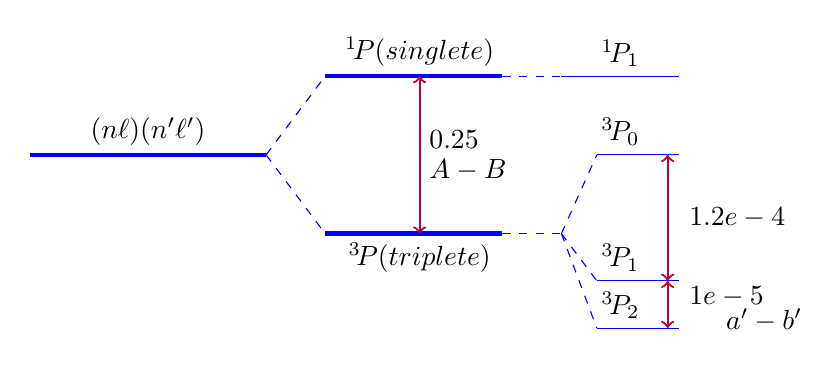
\begin{tikzpicture}[xscale=1.5,yscale=1]
        \draw node [above] at (0,1) {$(n\ell)(n'\ell')$};
        \draw[blue, ultra thick] (-1,1) -- (1,1);
        \draw[blue, thin, dashed] (1,1) -- (1.5,2);
        \draw[blue, thin, dashed] (1,1) -- (1.5,0);
        \draw[blue, ultra thick] (1.5,2) -- (3,2);
        \draw node [above] at (2.3,2) {${}^1\!P \text{ (singlete)}$};
        \draw[blue, ultra thick] (1.5,0) -- (3,0);
        \draw node [below] at (2.3,0) {${}^3\!P \text{ (triplete)}$};
        \draw[blue, thin, dashed] (3,2) -- (3.5,2);
        \draw[blue, thin] (3.5,2) -- (4.5,2);
        \draw node [above] at (4,2) {${}^1\!P_1$};
        \draw[blue, thin, dashed] (3,0) -- (3.5,0);
        \draw[blue, thin, dashed] (3.5,0) -- (3.8,1);
        \draw[blue, thin, dashed] (3.5,0) -- (3.8,-0.6);
        \draw[blue, thin, dashed] (3.5,0) -- (3.8,-1.2);
        %
        \draw[blue, thin] (3.8,1) --  (4.5,1)    ;
        \draw node [above] at (4,1) {${}^3\!P_0$};
        \draw[blue, thin] (3.8,-0.6) -- (4.5,-0.6)    ;
        \draw node [above] at (4,-0.6) {${}^3\!P_1$};
        \draw[blue, thin] (3.8,-1.2) -- (4.5,-1.2)    ;
        \draw node [above] at (4,-1.2) {${}^3\!P_2$};
        %
        \draw[purple,thick , <->] (2.3,2) -- (2.3,0);
        \draw node [right] at (2.3,1.2) {$\SI{0.25}{\eV}$};
        \draw node [right] at (2.3,0.8) {$A-B$};
        %
        \draw[purple,thick , <->] (4.4,1) -- (4.4,-0.6);
        \draw node [right] at (4.5,0.2) {$\SI{1.2e-4}{\eV}$};
        %
        \draw[purple,thick , <->] (4.4,-0.6) -- (4.4,-1.2);
        \draw node [right] at (4.5,-1.1) {$\ \ \ \ a'-b'$};
        \draw node [right] at (4.5,-0.8) {$\SI{1e-5}{\eV}$};
    \end{tikzpicture}
  \end{center}
  \caption{Degeneración de los niveles $(1s)(2s)$ del helio}
  \label{fig:heliumlevelfinal}
\end{figure}

\jokemargin{Y con esto y un bizcocho,
  hemos acabado el átomo de helio.}


%%% Local Variables:
%%% mode: latex
%%% TeX-master: "../resumen"
%%% End:
